\chaptersection{6}{Threat Scenarios e Threat Trees}

A partire dalla prioritizzazione sviluppata nel Capitolo 5 vengono approfonditi gli scenari di attacco maggiormente rappresentativi per DermaTriage. La selezione considera il livello di rischio ottenuto, il potenziale impatto sul sistema e la necessità di rappresentare superfici di attacco differenti della pipeline.

In particolare, vengono analizzate quattro minacce: la manipolazione intenzionale dell'immagine dermatologica, l'inserimento di contenuti avversariali nel feedback clinico, l'alterazione delle regole dell'Adaptation Layer e l'esposizione non autorizzata dei dati clinici. Tali scenari coprono rispettivamente la fase di input, il ciclo di aggiornamento, la logica decisionale finale e la protezione
delle informazioni sensibili.

Per ciascuna minaccia viene descritto uno scenario realistico compatibile con l'architettura analizzata e viene successivamente costruito un threat tree. La radice rappresenta l'obiettivo dell'attaccante, mentre i rami descrivono modalità alternative o condizioni concorrenti attraverso cui la minaccia può essere realizzata. Le foglie identificano infine le principali precondizioni o capability necessarie per completare il percorso di attacco.

\subsection{FM01.4 - Manipolazione intenzionale dell'immagine}
Un attaccante tenta di alterare il risultato del triage facendo elaborare a DermaTriage un'immagine dermatologica intenzionalmente manipolata. La compromissione può avvenire direttamente in fase di input, intervenendo sull'immagine prima dell'invio attraverso B4 o l'endpoint \texttt{/analyze}, oppure durante le successive fasi di trasferimento e preparazione dell'immagine prima dell'inferenza.

L'immagine modificata può influenzare EfficientNet-B4 introducendo perturbazioni capaci di alterare la classificazione iniziale dell'urgenza. Parallelamente, nel ramo multimodale, contenuti visivi appositamente costruiti possono influenzare Qwen2-VL e determinare una descrizione clinica non corrispondente alle caratteristiche reali della lesione. Tale alterazione può propagarsi agli stadi successivi della pipeline, influenzando BioMistral e, infine, la priorità clinica P1-P4 prodotta dall'Adaptation Layer.

\subsubsection{Threat tree}
Il threat tree rappresenta le principali modalità attraverso cui può materializzarsi FM01.4. La radice coincide con la minaccia di \textit{manipolazione intenzionale dell'immagine}, mentre i quattro rami
principali sono collegati tramite una relazione OR, poiché ciascuno di essi può costituire un percorso sufficiente per compromettere l'input visivo elaborato dalla pipeline.

\begin{figure}[htbp]
    \centering
    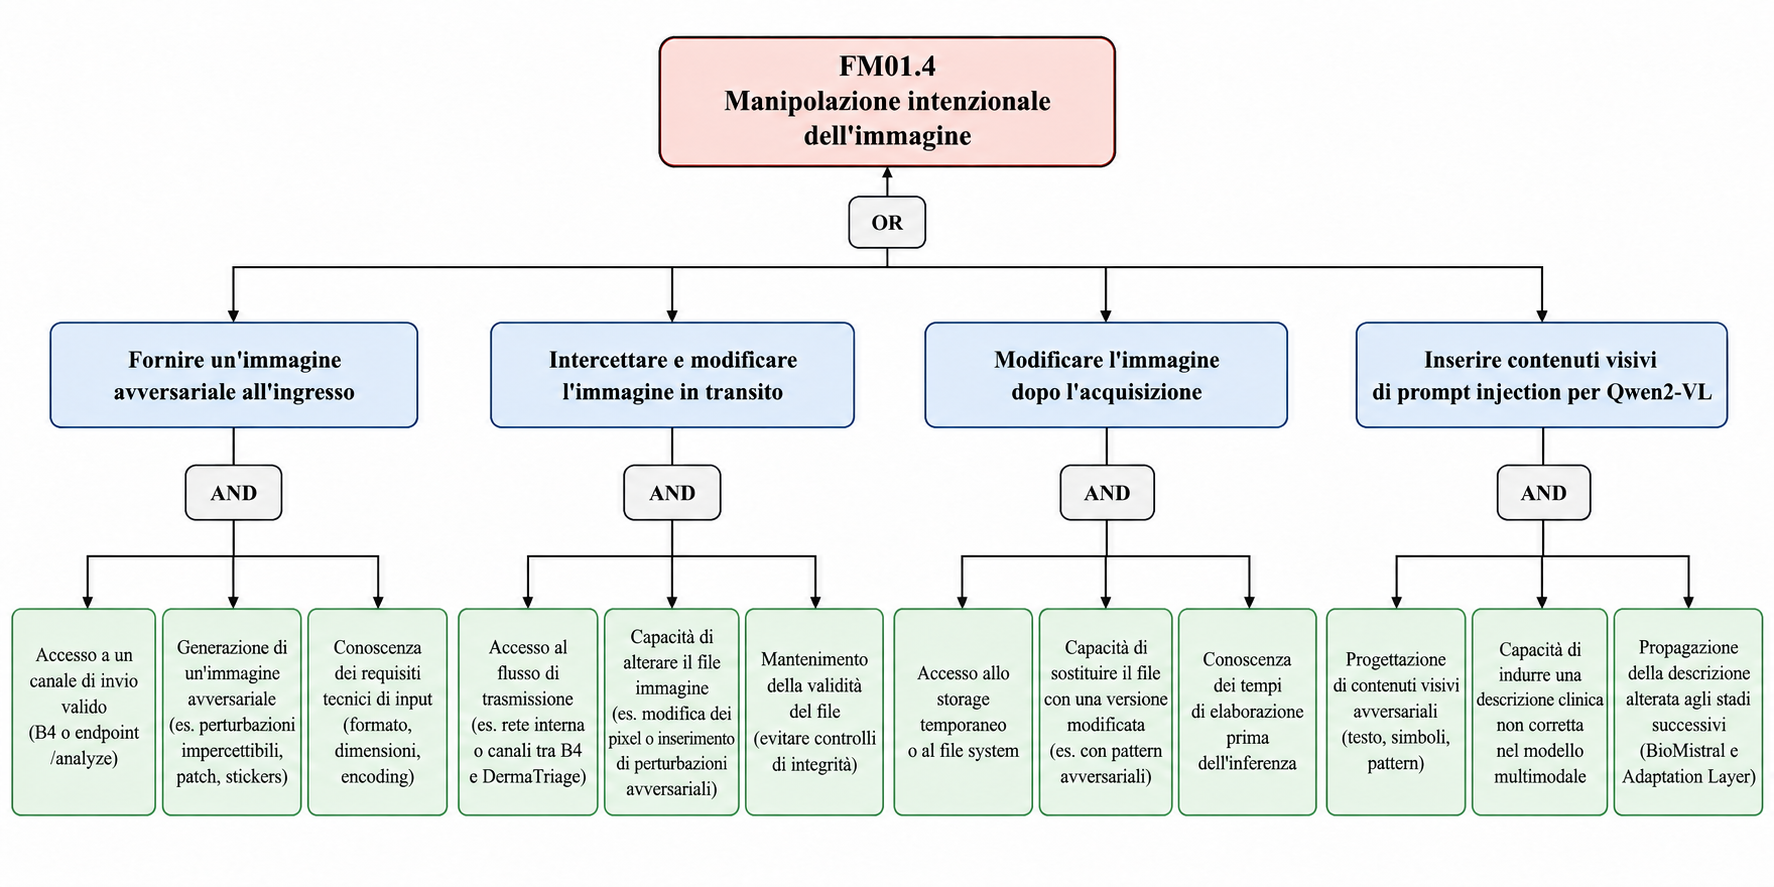
\includegraphics[width=\textwidth]{../Immagini/Threat Tree FM01-4.png}
    \caption{Threat tree relativo a FM01.4 - Manipolazione intenzionale dell'immagine}
    \label{fig:threat-tree-fm01-4}
\end{figure}

Il primo percorso considera l'invio diretto di un'immagine avversariale attraverso un canale di input valido, previa conoscenza dei requisiti tecnici richiesti dalla pipeline. Il secondo riguarda l'intercettazione e la modifica dell'immagine durante il trasferimento verso DermaTriage, mantenendo il file formalmente valido e utilizzabile dal sistema.

Il terzo percorso considera invece la modifica dell'immagine dopo l'acquisizione, attraverso l'accesso allo storage temporaneo o al file system utilizzato prima dell'inferenza. Il quarto riguarda specificamente Qwen2-VL e la possibilità di inserire nell'immagine contenuti visivi avversariali in grado
di influenzare l'interpretazione del modello multimodale e propagare una descrizione alterata verso BioMistral e l'Adaptation Layer.

I diversi percorsi non sono necessariamente esclusivi. Una stessa immagine può, ad esempio, contenere perturbazioni rivolte a EfficientNet-B4 e componenti visive progettate per influenzare Qwen2-VL. Il threat tree evidenzia quindi le principali precondizioni e capability richieste all'attaccante.

\subsection{FM13.1 - Contenuti avversariali nel feedback clinico}
Un attaccante riesce a introdurre nel feedback clinico contenuti progettati per influenzare i successivi meccanismi di aggiornamento della pipeline. Il feedback può apparire formalmente valido e coerente con una revisione clinica, pur contenendo istruzioni o pattern semantici avversariali destinati a essere
riutilizzati nel processo di evoluzione dei prompt.

La minaccia può manifestarsi sia attraverso l'inserimento iniziale di un feedback manipolato, sia mediante la modifica di una revisione già registrata. Se il contenuto contaminato viene successivamente selezionato dal processo di aggiornamento e incorporato in una nuova versione del prompt, l'effetto può
persistere nel tempo e influenzare le successive elaborazioni di Qwen2-VL o BioMistral.

\subsubsection{Threat tree}
La radice del threat tree coincide con la minaccia \textit{FM13.1 - Contenuti avversariali nel feedback clinico}. I tre rami principali sono collegati tramite una relazione OR e rappresentano modalità alternative attraverso cui il contenuto avversariale può essere introdotto, modificato o fatto entrare nel processo di aggiornamento dei prompt.

\begin{figure}[htbp]
    \centering
    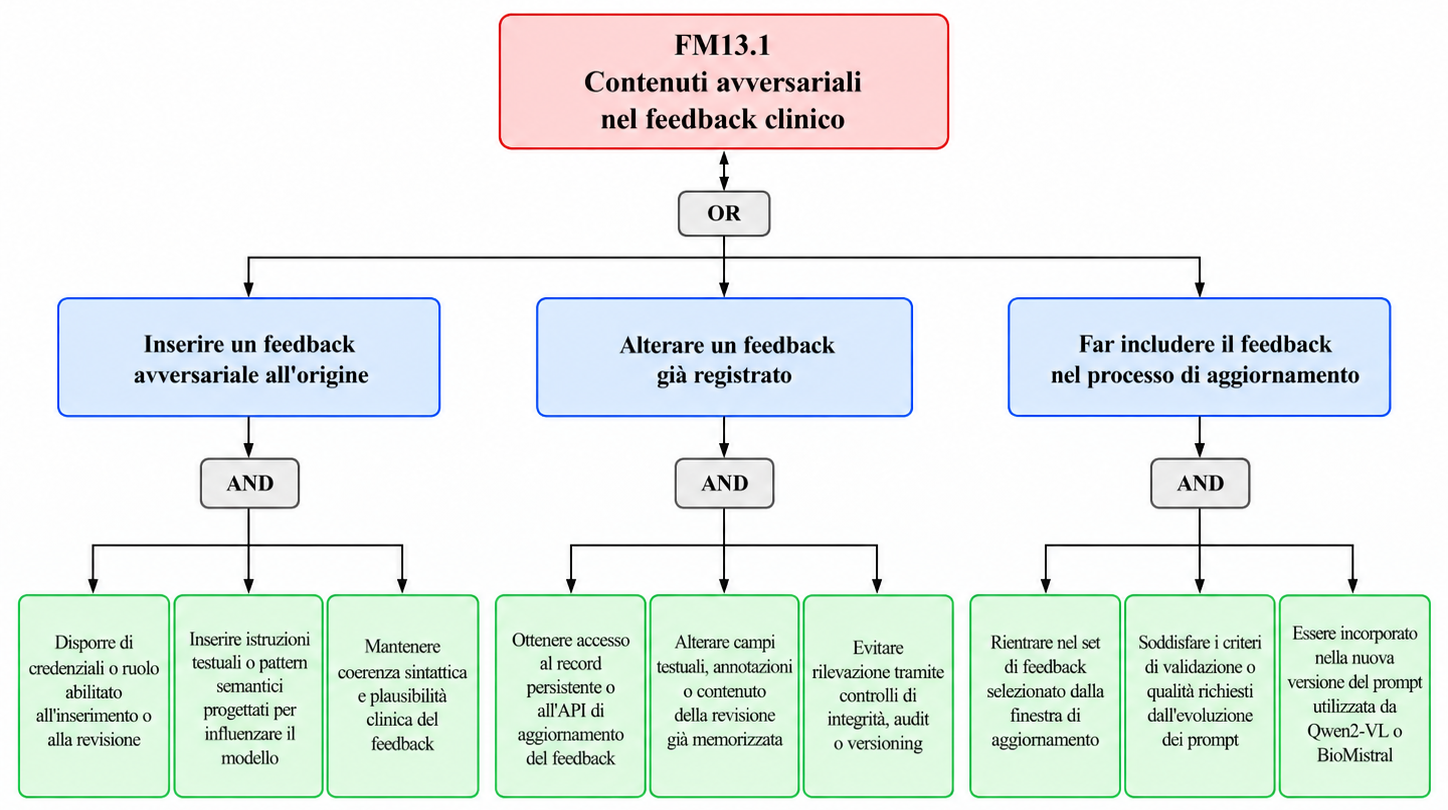
\includegraphics[width=\textwidth]{../Immagini/Threat Tree FM13-1.png}
    \caption{Threat tree relativo a FM13.1 - Contenuti avversariali nel feedback clinico}
    \label{fig:threat-tree-fm13-1}
\end{figure}

Il primo percorso riguarda l'inserimento diretto di un feedback avversariale all'origine. L'attaccante deve disporre di credenziali o di un ruolo che consenta l'inserimento o la revisione del feedback, costruire contenuti capaci di influenzare il comportamento dei modelli e mantenere al tempo stesso una
plausibilità sintattica e clinica sufficiente a non rendere immediatamente evidente la manipolazione.

Il secondo percorso considera l'alterazione di un feedback già registrato. In questo caso è necessario ottenere accesso al record persistente o alle API di aggiornamento, modificare i campi rilevanti della revisione e superare eventuali meccanismi di controllo dell'integrità, audit o versionamento.

Il terzo percorso riguarda il passaggio del feedback contaminato nel processo di evoluzione dei prompt. Il contenuto deve rientrare nel set selezionato dalla finestra di aggiornamento, soddisfare i criteri previsti dal processo di evoluzione e venire infine incorporato nella nuova versione del prompt 
utilizzata da Qwen2-VL o BioMistral.

Il threat tree evidenzia quindi come la minaccia possa derivare da percorsi differenti ma convergere nello stesso effetto: l'utilizzo persistente di contenuti contaminati nel ciclo di aggiornamento della pipeline.

\subsection{FM20.3 - Alterazione delle regole dell'Adaptation Layer}
Un attaccante riesce a modificare intenzionalmente le regole utilizzate dall'Adaptation Layer per convertire il livello di urgenza prodotto dalla pipeline nella priorità clinica P1-P4. La compromissione può riguardare direttamente la logica di mapping, i parametri decisionali utilizzati dalla funzione oppure la versione delle regole caricata ed eseguita dal sistema.

La modifica può lasciare invariati gli stadi di inferenza precedenti: EfficientNet-B4, Qwen2-VL e BioMistral possono quindi produrre risultati formalmente corretti, mentre l'Adaptation Layer li converte secondo regole alterate. Il sistema può continuare ad apparire operativo pur assegnando in modo sistematico priorità, specialisti o SLA differenti da quelli previsti, con possibili conseguenze dirette sulla presa in carico del paziente.

\subsubsection{Threat tree}
La radice del threat tree coincide con la minaccia \textit{FM20.3 - Alterazione intenzionale delle regole dell'Adaptation Layer}. I tre rami principali sono collegati tramite una relazione OR e rappresentano modalità alternative attraverso cui l'attaccante può compromettere la logica decisionale finale.

\begin{figure}[htbp]
    \centering
    
\includegraphics[width=\textwidth]{../Immagini/Threat Tree FM20-3.png}
    \caption{Threat tree relativo a FM20.3 - Alterazione intenzionale delle regole dell'Adaptation Layer}
    \label{fig:threat-tree-fm20-3}
\end{figure}

Il primo percorso riguarda la modifica diretta della logica di mapping. L'attaccante deve ottenere accesso al componente applicativo o al repository del codice, modificare le corrispondenze tra i livelli di urgenza HIGH/MEDIUM/LOW e le priorità P1--P4 e rendere operativa la versione alterata, ad esempio attraverso il normale meccanismo di deploy o il riavvio del servizio.

Il secondo percorso interessa i parametri decisionali utilizzati dall'Adaptation Layer, come la soglia di confidence impiegata per distinguere i casi HIGH assegnati a P1 da quelli assegnati a P2. La compromissione richiede l'individuazione dei parametri rilevanti, la modifica dei relativi valori nella
configurazione o nella risorsa in cui sono memorizzati e il mantenimento di una configurazione formalmente valida, così da evitare errori immediatamente rilevabili.

Il terzo percorso consiste nel caricamento di una versione non autorizzata delle regole. In questo caso, l'attaccante deve ottenere l'accesso al meccanismo di aggiornamento di tali regole o configurazioni, al fine di iniettare un artefatto contenente la logica alterata e indurre il sistema ad adottarlo, eludendo i controlli di integrità o provenienza.

I tre percorsi convergono nello stesso effetto: un risultato di inferenza correttamente prodotto può essere trasformato in una priorità clinica non corrispondente alle regole previste. Poiché l'output può rimanere formalmente valido, la compromissione può risultare difficile da individuare e influenzare più richieste di triage prima di essere rilevata.

\subsection{FM21.5 - Esposizione non autorizzata dei dati clinici}
Un attaccante riesce ad accedere senza autorizzazione alle informazioni cliniche associate ai consulti gestiti tramite B4 e utilizzati da DermaTriage. I dati potenzialmente esposti comprendono immagini dermatologiche, dati clinici e anagrafici, documenti allegati, risultati diagnostici e validazioni mediche.

La compromissione può derivare dall'uso improprio dei meccanismi di autenticazione, dallo sfruttamento di controlli di autorizzazione insufficienti oppure dall'accesso diretto alle risorse che memorizzano o trasportano i dati. In tutti questi casi, informazioni destinate esclusivamente a soggetti o componenti autorizzati possono essere consultate, estratte o intercettate da un attaccante, con impatto diretto sulla confidenzialità e sulla privacy del paziente.

\subsubsection{Threat tree}
La radice del threat tree coincide con la minaccia \textit{FM21.5 - Esposizione non autorizzata dei dati clinici}. I tre rami principali sono collegati tramite una relazione OR e rappresentano modalità alternative attraverso cui un attaccante può ottenere accesso a informazioni cliniche riservate.

\begin{figure}[htbp]
    \centering
    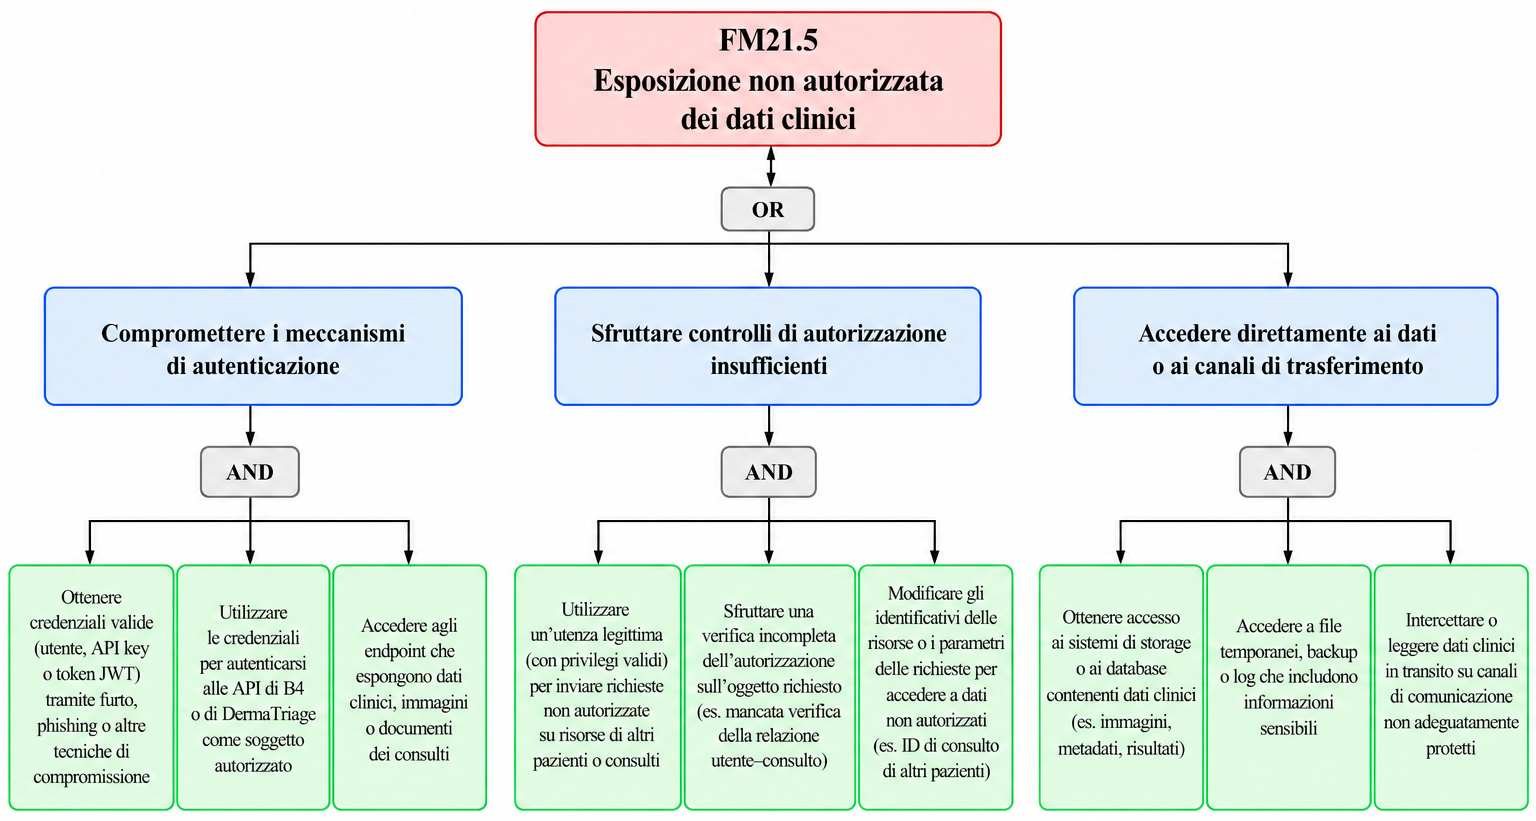
\includegraphics[width=\textwidth]{../Immagini/Threat Tree FM21-5.png}
    \caption{Threat tree relativo a FM21.5 - Esposizione non autorizzata dei dati clinici}
    \label{fig:threat-tree-fm21-5}
\end{figure}

Il primo percorso riguarda la compromissione dei meccanismi di autenticazione. L'attaccante deve ottenere credenziali valide, quali utenze, API key o token JWT, tramite furto, phishing o altre tecniche di compromissione, utilizzarle per autenticarsi alle API di B4 o di DermaTriage e accedere così agli endpoint che espongono dati clinici, immagini o documenti dei consulti.

Il secondo percorso considera lo sfruttamento di controlli di autorizzazione insufficienti. In questo caso l'attaccante opera come utente regolarmente autenticato, ma utilizza privilegi validi per inviare richieste non autorizzate su risorse riferite ad altri pazienti o consulti. La minaccia si concretizza quando il sistema applica verifiche incomplete sull'oggetto richiesto, ad esempio non controllando correttamente la relazione tra utente e consulto, oppure quando è possibile modificare identificativi o parametri della richiesta per accedere a dati non autorizzati.

Il terzo percorso riguarda l'accesso diretto ai dati o ai canali di trasferimento. L'attaccante può ottenere accesso ai sistemi di storage o ai database contenenti immagini, metadati e risultati, consultare file temporanei, backup o log che includono informazioni sensibili, oppure intercettare dati
clinici in transito su canali di comunicazione non adeguatamente protetti.

I tre percorsi convergono nella stessa conseguenza: informazioni cliniche sensibili vengono rese disponibili a soggetti non autorizzati. La portata dell'esposizione dipende dal livello di accesso ottenuto e può riguardare un singolo consulto oppure un insieme più ampio di dati gestiti dal sistema.